\documentclass[border=14pt]{standalone}
\usepackage[T1]{fontenc}
\usepackage[scaled=1.0]{helvet}
\renewcommand{\familydefault}{\sfdefault}
\usepackage{amsmath}
\usepackage{sansmath}
\sansmath
\hyphenpenalty=10000
\exhyphenpenalty=10000
\usepackage{xcolor}
\usepackage{tikz}
\usetikzlibrary{arrows.meta,positioning,calc,fit,backgrounds}
\definecolor{cblue}{HTML}{CFE2F8}
\definecolor{cpeach}{HTML}{F9DDD2}
\definecolor{cmint}{HTML}{D3EFE1}
\definecolor{cgrey}{HTML}{ECEBE7}
\definecolor{cline}{HTML}{6B6B6B}
\definecolor{clabel}{HTML}{555555}
\tikzset{
  blk/.style={draw=cline, line width=1.1pt, rounded corners=6pt, align=center, inner sep=6pt, minimum height=2.1cm, text width=#1},
  blk/.default=5.0cm,
  data/.style={blk=#1, fill=cgrey}, data/.default=5.0cm,
  ctrl/.style={blk=#1, fill=cblue}, ctrl/.default=5.0cm,
  path/.style={blk=#1, fill=cpeach}, path/.default=5.0cm,
  ana/.style={blk=#1, fill=cmint}, ana/.default=5.0cm,
  wire/.style={-{Stealth[length=9pt,width=7pt]}, draw=cline, line width=1.1pt},
  dwire/.style={wire, dashed},
  lab/.style={font=\normalsize, text=clabel},
  lane/.style={font=\large\bfseries, text=clabel},
}
\newcommand{\nt}[2]{{\LARGE #1}\\[3pt]{\Large #2}}

\begin{document}
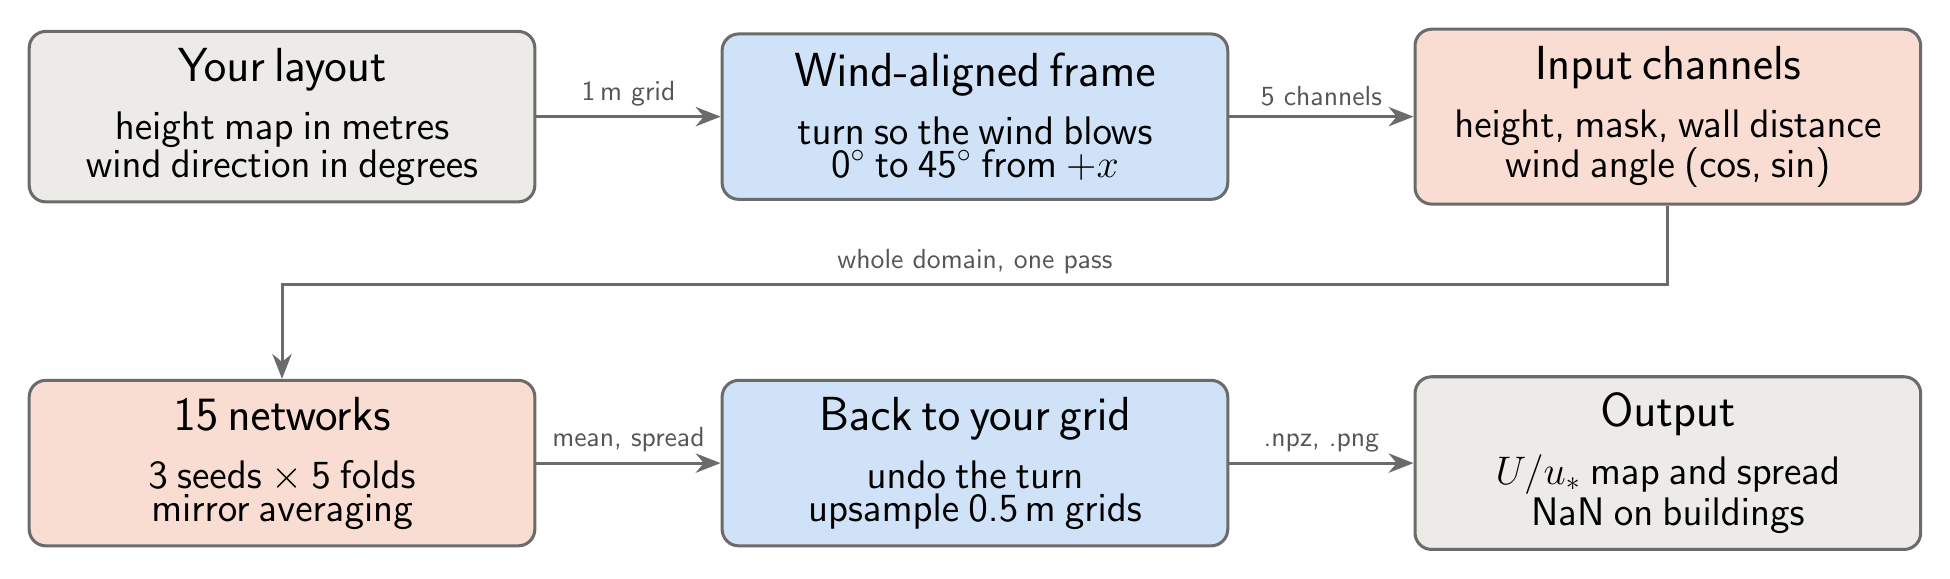
\begin{tikzpicture}
\def\dx{8.8}
\node[data=6.0cm] (in) at (0,0) {\nt{Your layout}{height map in metres\\wind direction in degrees}};
\node[ctrl=6.0cm] (fr) at (\dx,0) {\nt{Wind-aligned frame}{turn so the wind blows\\0$^\circ$ to 45$^\circ$ from $+x$}};
\node[path=6.0cm] (ch) at (2*\dx,0) {\nt{Input channels}{height, mask, wall distance\\wind angle (cos, sin)}};
\node[path=6.0cm] (nn) at (0,-4.4) {\nt{15 networks}{3 seeds $\times$ 5 folds\\mirror averaging}};
\node[ctrl=6.0cm] (bk) at (\dx,-4.4) {\nt{Back to your grid}{undo the turn\\upsample 0.5\,m grids}};
\node[data=6.0cm] (out) at (2*\dx,-4.4) {\nt{Output}{$U/u_*$ map and spread\\NaN on buildings}};
\draw[wire] (in) -- node[lab, above] {1\,m grid} (fr);
\draw[wire] (fr) -- node[lab, above] {5 channels} (ch);
\draw[wire] (ch.south) -- ++(0,-1.0) -| node[lab, pos=0.25, above] {whole domain, one pass} (nn.north);
\draw[wire] (nn) -- node[lab, above] {mean, spread} (bk);
\draw[wire] (bk) -- node[lab, above] {.npz, .png} (out);
\end{tikzpicture}
\end{document}
